
\documentclass[../main.tex]{subfiles}
\begin{document}

\chapter{Results and Analysis}
\label{ch:resultsAndAnalysis}

%\engExpl{Sometimes this is split into two chapters.\\Keep in mind: How you are going to evaluate what you have done? What are your metrics?\\Analysis of your data and proposed solution\\Does this meet the goals which you had when you started?}

In this chapter, we will present the project's main results and discuss them. The code, as well as additional results, can be found in the following GitHub repository: \url{https://github.com/AGarciaCast/Topo_Reg_Relative_Rep}


\section{Latent space similarity analysis}
\label{sec:res_lat}
\subsection{Autoencoder}
\subsubsection*{One linear layer and two-dimensional latent space}

In accordance with the experiment conducted in the original latent space paper \cite{moschella_relative_2022}, we will set the dimension of the latent space to two in order to visualize it without dimensionality reduction. Initially, we will explore the case where just one linear layer is used to transition from the convolutional feature map to the two-dimensional space.\\

As described in Section~\ref{sec:latent_meth}, we will employ the CKA metric to compare the latent representations of this network across different initializations. Figure~\ref{fig:cka_ae_2} displays the discrepancies between the representations generated by the encoder and decoder. Notably, there are instances, such as seed 42 vs. seed 121, where the differences in representations are more pronounced than those between seed 121 and seed 200. We attribute this phenomenon to the model's need to find the optimal linear transformation for reducing an 896-dimensional space to a 2-dimensional one. Considering that the optimal solution in terms of MSE corresponds to the PCA embedding, we believe that the variation in representations may arise from using a different basis than the eigenvectors for dimensionality reduction. Consequently, when encoded using distinct approximations of the principal component, the decoder latent spaces will differ.\\

\begin{figure}[ht!]
     \centering
    \begin{subfigure}[b]{0.45\textwidth}
         \centering
        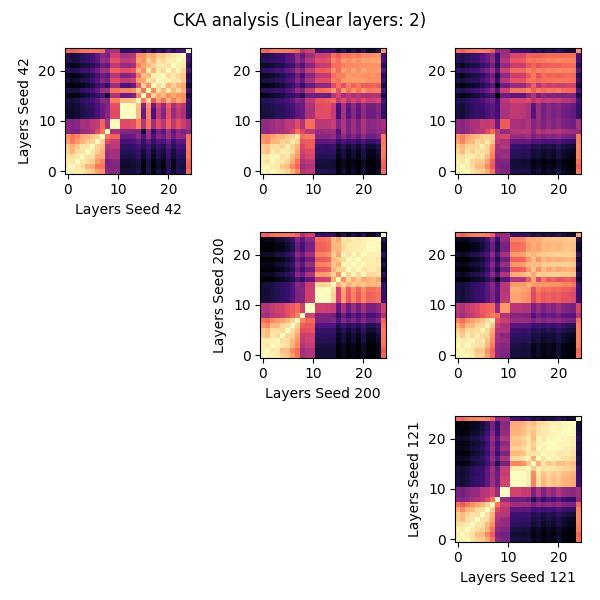
\includegraphics[width=\textwidth]{figures/rs/sim_ae/cka_2__42_200_121.png} 
        \caption{CKA analysis}
        \label{fig:cka_ae_2}
     \end{subfigure}\hfill
      \begin{subfigure}[b]{0.45\textwidth}
         \centering
         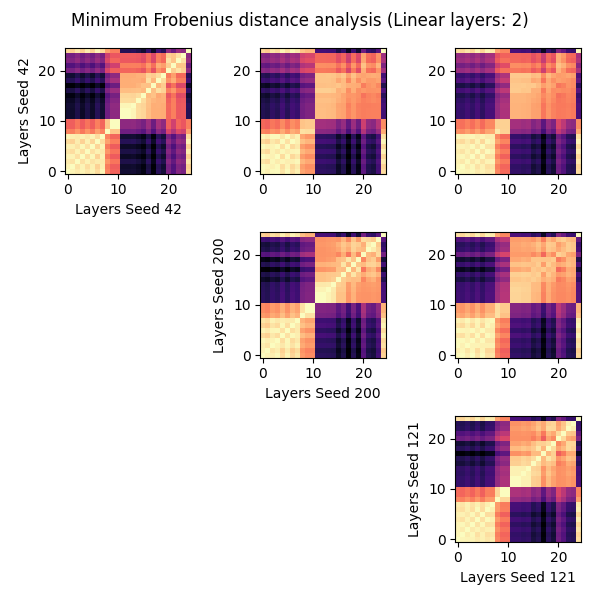
\includegraphics[width=\textwidth]{figures/rs/sim_ae/frob_2__42_200_121.png}
        \caption{Min. Frobenius norm}
         \label{fig:frob_ae_2}
     \end{subfigure}
    \caption{Numerical latent space analysis for the autoencoder with linear layers: 2}
    \label{fig:lat_num_ae_2}
\end{figure}

Figure~\ref{fig:frob_ae_2} illustrates that the previously obtained results using CKA align with those derived from measuring the minimum Frobenius distance between the $L^2$ distance matrices.

\begin{figure}[ht!]
    \centering
    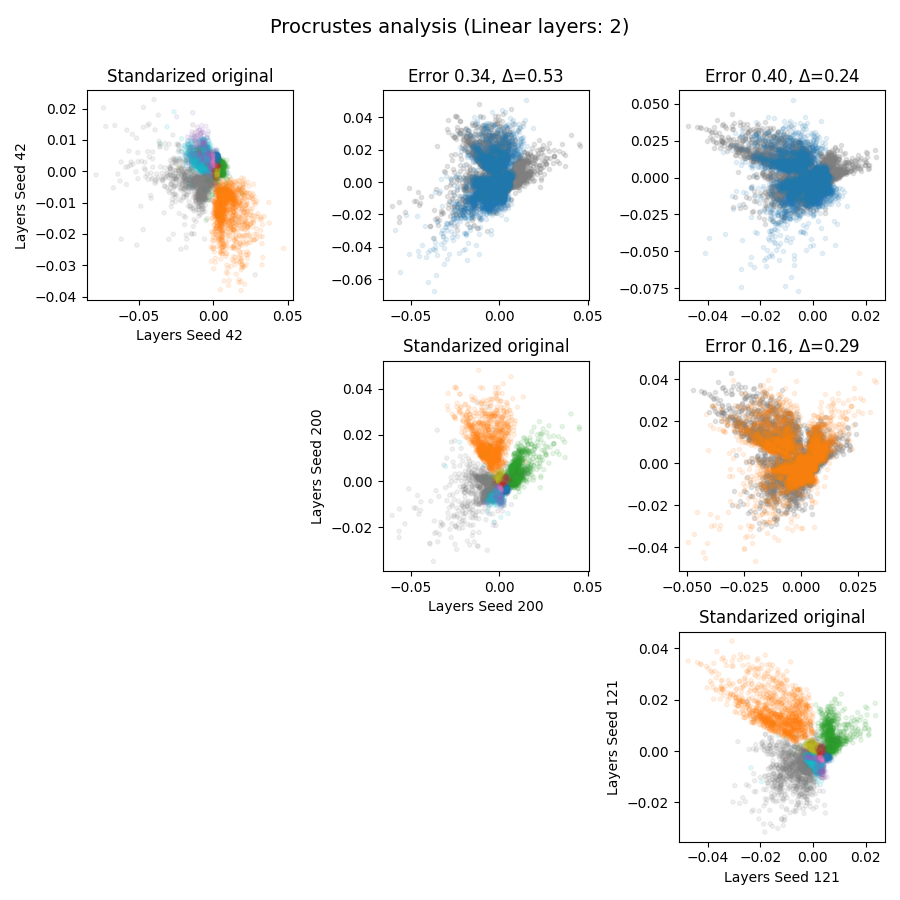
\includegraphics[width=0.7\textwidth]{figures/rs/sim_ae/procrustes_2__42_200_121.png} 
    \caption{Procrustes analysis for the autoencoder with linear layers: 2}
    \label{fig:proc_ae_2}
\end{figure}


Furthermore, we will employ Procrustes analysis to visually validate the similarity of these representations by examining their overlap after applying the optimal isometry up-to-scale transformation in terms of MSE. The interpretation of the Procrustes analysis presented in Figure~\ref{fig:proc_ae_2} is as follows:
\begin{enumerate}
    \item The diagonal elements represent the original 2-dimensional latent space generated by the encoder, with each class indicated by a distinct color.
    \item Column-wise, we fix the original latent representation as our reference and plot it in the background in grey.
    \item Row-wise, we apply the optimal Procrustes transformation to minimize the Procrustes error with respect to the fixed column reference. The transformed space is then colored.
    \item We show the Procrustes error, as well as the Frobenius distance between the applied optimal orthogonal Procrustes transformation and the optimal permutation Procrustes transformation (denoted by $\Delta$). The latter indicates the degree to which we deviate from a theoretical intertwiner group a action.
\end{enumerate}

Hence, Figure~\ref{fig:proc_ae_2} reveals that cases with higher numerical similarity correspond to smaller Procrustes errors. Even when higher Procrustes errors are observed, some similarities can still be observed between the two overlapping representations, suggesting the potential use of other metrics commonly employed in image segmentation, such as Jaccard or Dice coefficients.

Regarding the distance to the optimal permutation matrix, we lack sufficient evidence to confirm whether it comes from the intertwiner group or is simply an artifact resulting from finding sub-optimal approximations of principal components.\\

\begin{mathNote}
In Appendix~\ref{sec:add_lat}, we present the numerical and Procrustes analysis results for two additional seeds for all the setups utilized in Section~\ref{sec:res_lat}. It is important to note that these supplementary results align with those presented using only three seeds.
\end{mathNote}

\subsubsection*{Multiple linear layers and two-dimensional latent space}

In this case, we will employ the following Multi-Layer Perceptron (MLP) architecture to transition from the convolutional feature map to the 2-dimensional space: 512-256-128-32-2. This choice ensures that any similarities observed in the linear layers are not solely attributed to the inductive bias of the convolutional layers.\\

\begin{figure}[ht!]
     \centering
    \begin{subfigure}[b]{0.45\textwidth}
         \centering
        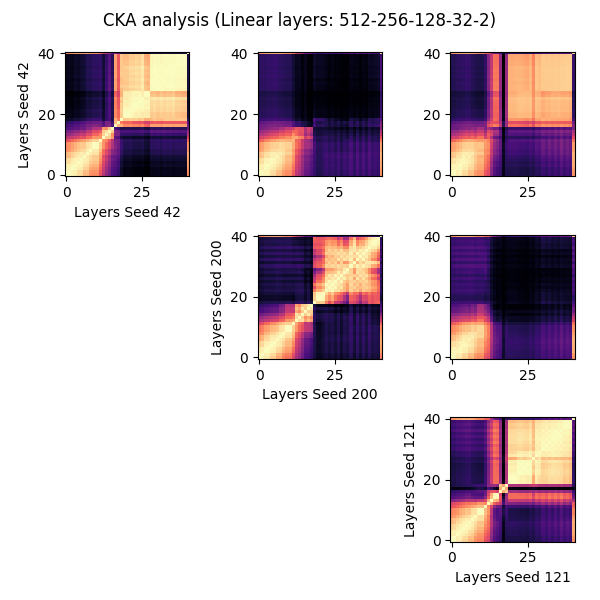
\includegraphics[width=\textwidth]{figures/rs/sim_ae/cka_512-256-128-32-2__42_200_121.png} 
        \caption{CKA analysis}
        \label{fig:cka_ae_512_256_128_32_2}
     \end{subfigure}\hfill
      \begin{subfigure}[b]{0.45\textwidth}
         \centering
         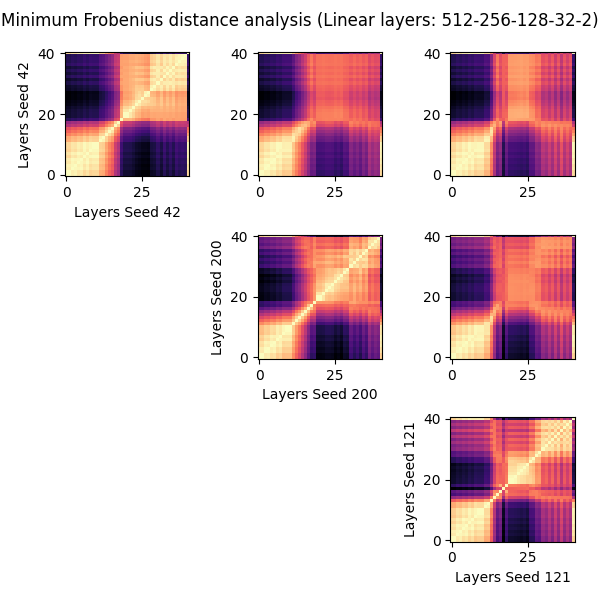
\includegraphics[width=\textwidth]{figures/rs/sim_ae/frob_512-256-128-32-2__42_200_121.png}
        \caption{Min. Frobenius norm}
         \label{fig:frob_ae_512_256_128_32_2}
     \end{subfigure}
    \caption{Numerical latent space analysis for the autoencoder with linear layers: 512-256-128-32-2}
    \label{fig:lat_num_ae_512_256_128_32_2}
\end{figure}

Figures~\ref{fig:cka_ae_512_256_128_32_2},~\ref{fig:extra_cka_ae_512_256_128_32_2} show that in this case, we obtain can obtain somewhat different representations in terms of CKA. However, the min Frobenius distance (Figures~\ref{fig:frob_ae_512_256_128_32_2},~\ref{fig:extra_frob_ae_512_256_128_32_2}) indicate that there might be a slight similarity. So this gives us the understanding that CKA can be more ``pessimistic'' than the Frobenius distance. Nevertheless, we still see a correlation between the results of the CKA plots and the Frobenius ones.\\

We believe that the reason for obtaining more distinct representations when employing the AE architecture lies in the multiple ways that exist to incorrectly map an 896-dimensional space to a 2-dimensional one using a highly expressive non-linear function. Consequently, Figure~\ref{fig:proc_ae_512_256_128_32_2} illustrates collapsed class clusters and excessive spread in certain cases. Notably, some of these issues could potentially be mitigated by utilizing a Variational Autoencoder (VAE) since it applies proper regularization to the encoded space.\\

Lastly, we can see in Figure~\ref{fig:proc_ae_512_256_128_32_2} that the case where we obtained the best similarity in terms of CKA, we also obtain the smallest Procrustes error. Furthermore, we can observe that our findings based on the Frobenius norm were not entirely inaccurate, as there are local resemblances between the latent spaces (e.g., dispersion patterns in the blue and orange classes).

\begin{figure}[ht!]
    \centering
    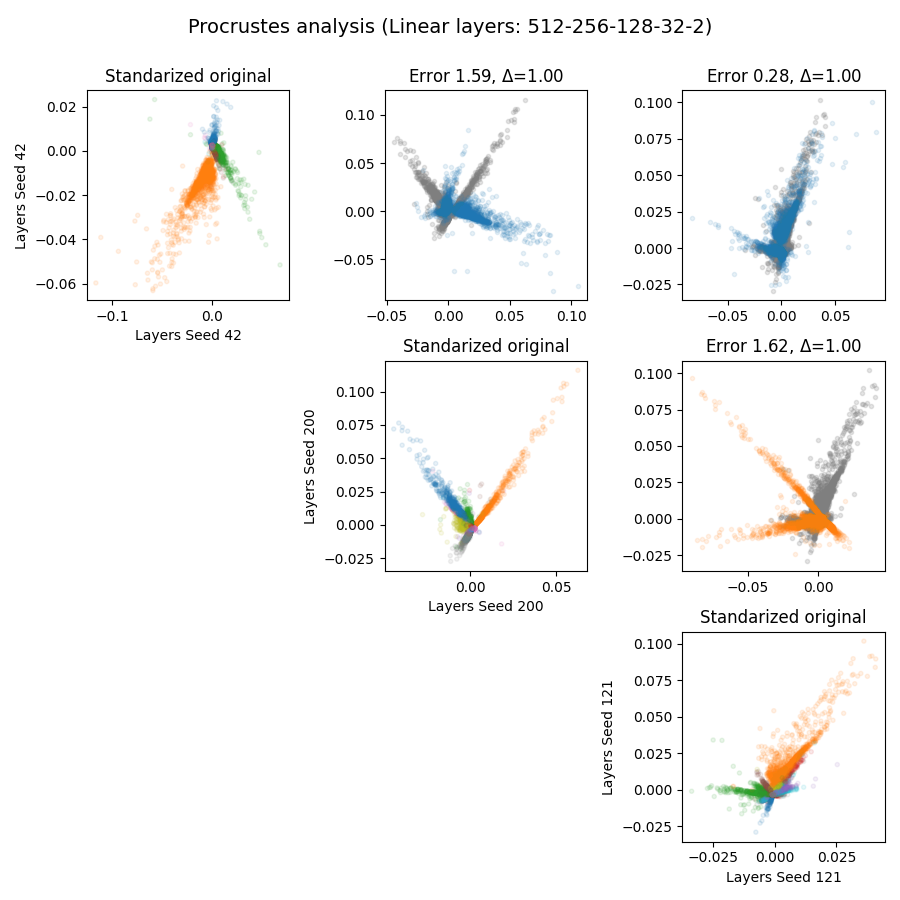
\includegraphics[width=0.7\textwidth]{figures/rs/sim_ae/procrustes_512-256-128-32-2__42_200_121.png} 
    \caption{Procrustes analysis for the autoencoder with linear layers: 512-256-128-32-2}
    \label{fig:proc_ae_512_256_128_32_2}
\end{figure}


\subsubsection*{Multiple linear layers and high-dimensional latent space}
We will explore the final configuration of the Autoencoder, which utilizes multiple linear layers to transition from the convolutional feature map to a 32-dimensional space: 512-256-128-32. This choice is motivated by the assertion made in \cite{kornblith_similarity_2019} that "well-performing" networks yield more similar representations. Hence, we aim to investigate whether these networks also tend to produce representations that are $\epsilon$-similar.\\

Figure~\ref{fig:lat_num_ae_512_256_128_32} supports this claim, as we observe high similarities in terms of both CKA and the Frobenius norm. We believe that this outcome may be attributed to the fact that autoencoders with a higher-dimensional latent space exhibit greater simplicity, as they lack a strong information bottleneck.\\


\begin{figure}[ht!]
     \centering
    \begin{subfigure}[b]{0.45\textwidth}
         \centering
        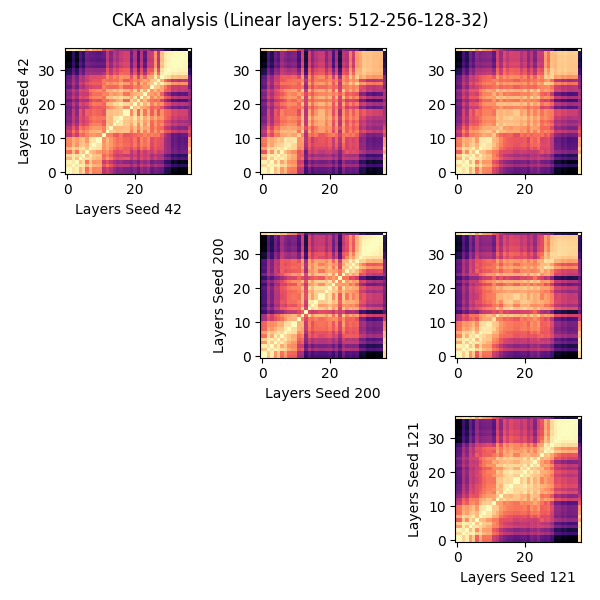
\includegraphics[width=\textwidth]{figures/rs/sim_ae/cka_512-256-128-32__42_200_121.png} 
        \caption{CKA analysis}
        \label{fig:cka_ae_512_256_128_32}
     \end{subfigure}\hfill
      \begin{subfigure}[b]{0.45\textwidth}
         \centering
         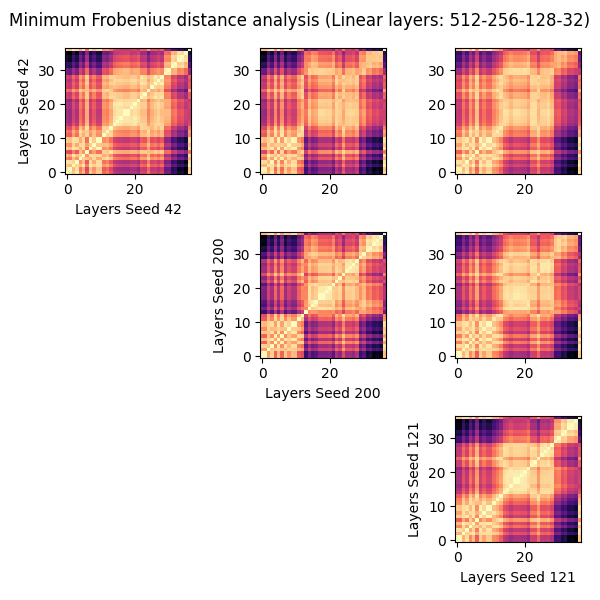
\includegraphics[width=\textwidth]{figures/rs/sim_ae/frob_512-256-128-32__42_200_121.png}
        \caption{Min. Frobenius norm}
         \label{fig:frob_ae_512_256_128_32}
     \end{subfigure}
    \caption{Numerical latent space analysis for the autoencoder with linear layers: 512-256-128-32}
    \label{fig:lat_num_ae_512_256_128_32}
\end{figure}


\begin{figure}[ht!]
    \centering
    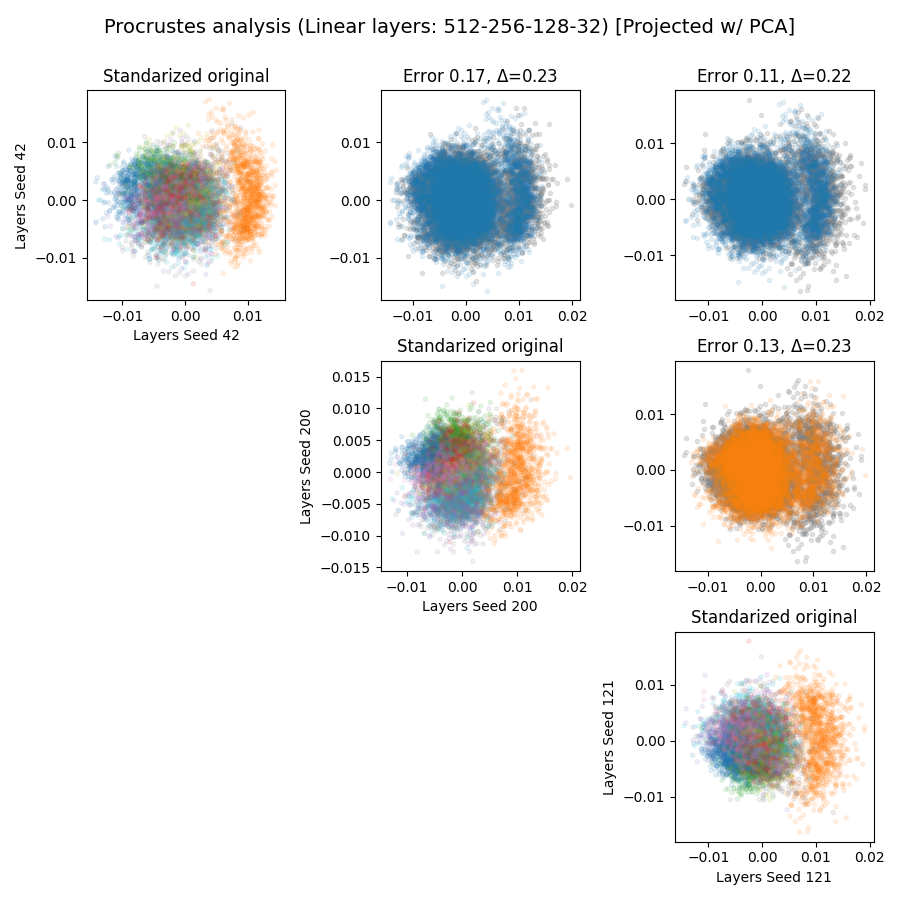
\includegraphics[width=0.7\textwidth]{figures/rs/sim_ae/procrustes_512-256-128-32__42_200_121.png} 
    \caption{Procrustes analysis for the autoencoder with linear layers: 512-256-128-32}
    \label{fig:proc_ae_512_256_128_32}
\end{figure}

Since we now possess a high-dimensional latent space, additional dimensionality reduction techniques are necessary for visualization purposes. We have opted to employ Principal Component Analysis (PCA) because, as depicted in Figure~\ref{fig:tsne_ae_512_256_128_32}, t-SNE may not produce encodings that lend themselves to a clear understanding of the effects of Procrustes analysis. However, even with PCA, Figure~\ref{fig:proc_ae_512_256_128_32} reveals that the resulting representation is suboptimal for this task, as numerous clusters exhibit significant overlap in their projections.


\subsection{Classifier}
As previously described, we will repeat the previous experiment using now a simple CNN on a classification task.\\

\begin{figure}[ht!]
     \centering
    \begin{subfigure}[b]{0.45\textwidth}
         \centering
        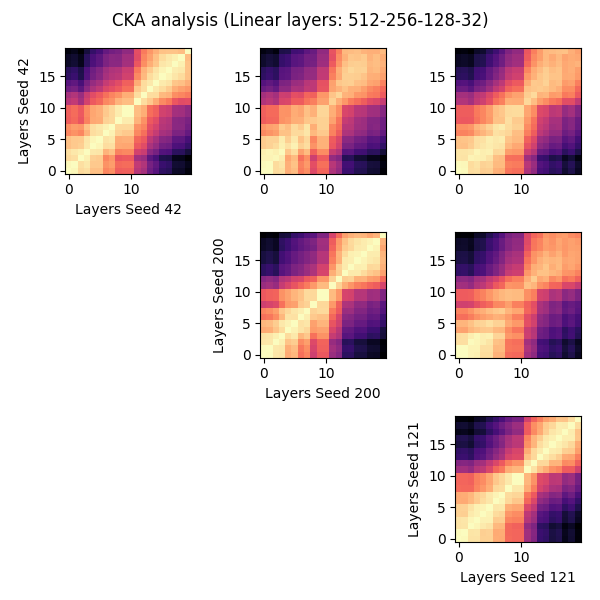
\includegraphics[width=\textwidth]{figures/rs/sim_cls/cka_512-256-128-32__42_200_121.png} 
        \caption{CKA analysis}
        \label{fig:cka_cls}
     \end{subfigure}\hfill
      \begin{subfigure}[b]{0.45\textwidth}
         \centering
         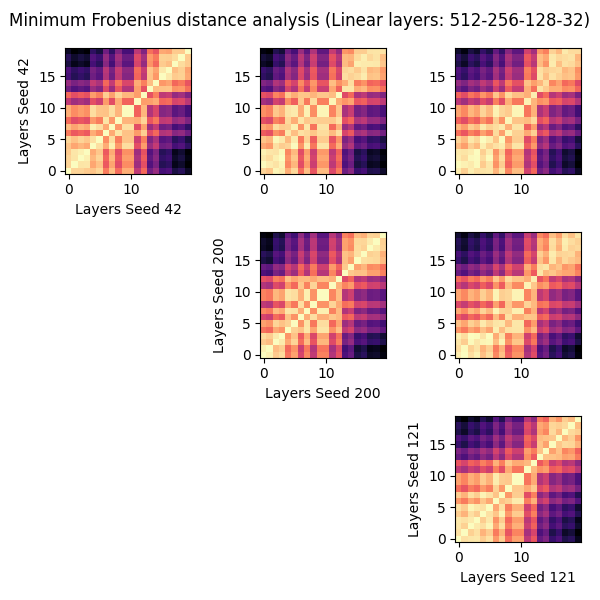
\includegraphics[width=\textwidth]{figures/rs/sim_cls/frob_512-256-128-32__42_200_121.png}
        \caption{Min. Frobenius norm}
         \label{fig:frob_cls}
     \end{subfigure}
    \caption{Numerical latent space analysis for the CNN classifier}
    \label{fig:lat_num_cls}
\end{figure}

As depicted in Figure~\ref{fig:lat_num_cls}, we observe significant similarities in terms of both CKA and the Frobenius norm. Consequently, we have obtained empirical evidence supporting the existence of $\epsilon$-similarities in the context of a classification task. It is important to note that the original paper just provided numerical analysis on word embeddings and visual examples on Autoencoders and ViTs..\\

Furthermore, we conducted Procrustes analysis on the latent representations obtained from the vectorized convolutional feature map, positioned just before the classification head (see Figure~\ref{fig:proc_cls}). We chose this since this is the position where we will apply the relative transformations and topological regularization in the next subsections. \\


\begin{figure}[ht!]
    \centering
    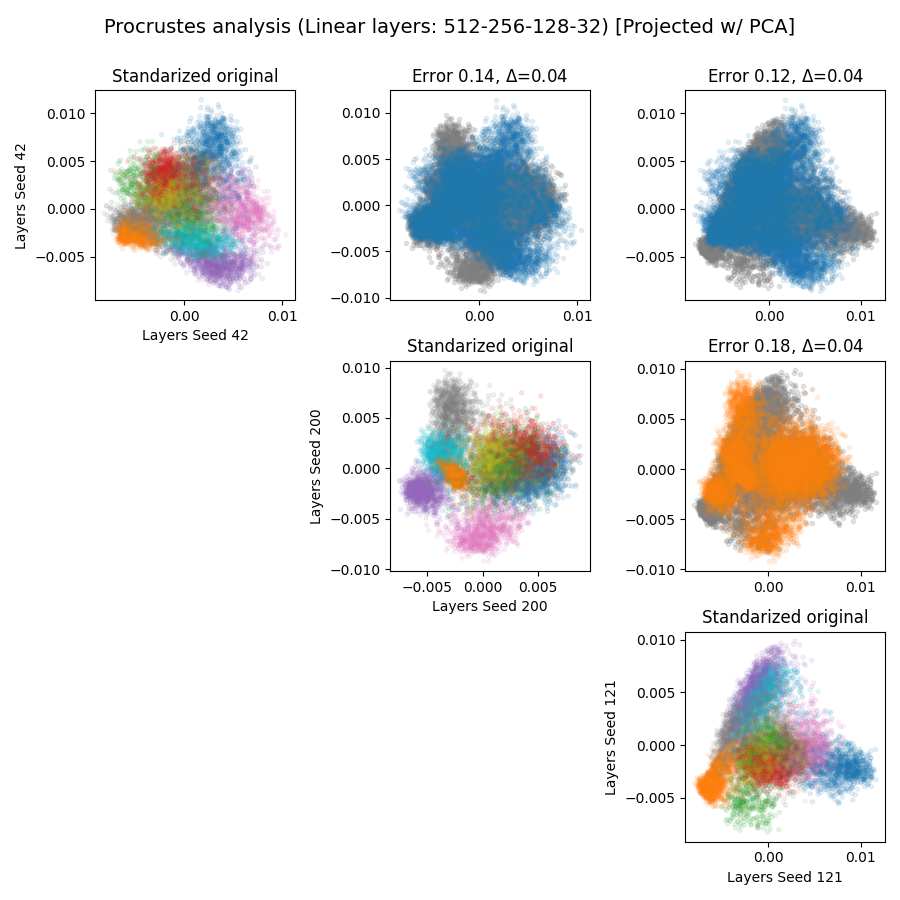
\includegraphics[width=0.7\textwidth]{figures/rs/sim_cls/procrustes_512-256-128-32__42_200_121.png} 
    \caption{Procrustes analysis for the CNN classifier}
    \label{fig:proc_cls}
\end{figure}

In conclusion, these empirical findings, combined with the new theoretical framework presented in Section~\ref{sec:latent_meth}, contribute to a deeper understanding of the potential causes of $\epsilon$-similarities, to which our relative transformations aim to be invariant. However, it is important to recognize that this is only a small piece of the larger puzzle that the field of Representation Similarity aims to assemble.

\section{Multilingual model stitching}

\subsection{Full fine-tuning analysis}

As discussed in Section~\ref{sec:topo_meth}, we have made some methodological changes from the original paper implementation of the following experiments. As a reference, the results presented in the original relative transformation paper are shown in Table~\ref{tab:multilingual-fine-tune-og}.\\

\begin{table}[ht!]
\centering
\resizebox{0.7\textwidth}{!}{
\begin{tabular}{clcccc}
\toprule
   &    & \multicolumn{2}{c}{Absolute} & \multicolumn{2}{c}{Relative} \\
 \cmidrule(lr){3-4} 
 \cmidrule(lr){5-6} 
 Decoder & Encoder & $\text{FScore} \times 100$ & MAE & $\text{FScore} \times 100$ & MAE \\
\midrule
\multirow{3}{*}{en} & en &  $65.46 \pm 2.89$ &  $0.38 \pm 0.02$ &  $61.18 \pm 1.92$ &  $0.44 \pm 0.02$ \\
   & es &  $22.70 \pm 0.41$ &  $1.39 \pm 0.03$ &  $51.67 \pm 1.20$ &  $0.62 \pm 0.01$ \\
   & fr &  $30.75 \pm 0.67$ &  $1.19 \pm 0.02$ &  $49.18 \pm 0.83$ &  $0.69 \pm 0.02$ \\
&\\
\multirow{3}{*}{es} & en &  $21.24 \pm 0.81$ &  $1.43 \pm 0.07$ &  $51.02 \pm 2.54$ &  $0.68 \pm 0.05$ \\
   & es &  $61.29 \pm 3.04$ &  $0.43 \pm 0.02$ &  $57.89 \pm 3.80$ &  $0.48 \pm 0.03$ \\
   & fr &  $29.02 \pm 0.85$ &  $1.26 \pm 0.05$ &  $48.40 \pm 1.02$ &  $0.71 \pm 0.02$ \\
&\\
\multirow{3}{*}{fr} & en &  $27.39 \pm 1.22$ &  $1.23 \pm 0.06$ &  $45.55 \pm 3.55$ &  $0.76 \pm 0.09$ \\
   & es &  $29.47 \pm 3.68$ &  $1.18 \pm 0.07$ &  $40.29 \pm 1.72$ &  $0.90 \pm 0.04$ \\
   & fr &  $56.40 \pm 1.89$ &  $0.51 \pm 0.01$ &  $53.58 \pm 0.70$ &  $0.57 \pm 0.01$ \\
\bottomrule
\end{tabular}
}
\caption{Summary of the original results presented in \cite{moschella_relative_2022} (over five random seeds)}
\label{tab:multilingual-fine-tune-og}
\end{table}

As shown in Table~\ref{tab:multilingual-fine-tune-fine-grained}, we observe slightly worst results when replicating the original training setup while incorporating our proposed methodological changes. However, as previously discussed, we will proceed with this new setup as it represents a more common methodology. Additionally, some of the introduced changes, such as employing gradient accumulation with smaller batch sizes, were necessary to train the models on our V100 GPU successfully. It would, however, be interesting to conduct further analysis to understand why the inclusion of post $L^2$ normalization on the relative transformation and the utilization of the ``non-standard'' classification head leads to improved performance.\\

\begin{table}[ht!]
\centering
\resizebox{\textwidth}{!}{
\begin{tabular}{clcccccc}
\toprule
   &    & \multicolumn{3}{c}{Absolute} & \multicolumn{3}{c}{Relative} \\
 \cmidrule(lr){3-5} 
 \cmidrule(lr){6-8} 
 Decoder & Encoder & $\text{Acc} \times 100$ & $\text{FScore} \times 100$ & $\text{MAE} \times 100$ & $\text{Acc} \times 100$ & $\text{FScore} \times 100$ & $\text{MAE} \times 100$ \\
\midrule
\multirow{3}{*}{en} & en &  $55.67 \pm 0.58$ &  $54.96 \pm 1.86$ &    $53.80 \pm 2.55$ &  $55.06 \pm 0.82$ &  $54.33 \pm 1.13$ &   $55.69 \pm 2.33$ \\
   & es &  $18.80 \pm 1.61$ &   $8.14 \pm 2.06$ &  $191.49 \pm 12.12$ &  $44.59 \pm 0.16$ &  $42.44 \pm 0.59$ &   $79.93 \pm 0.27$ \\
   & fr &  $21.30 \pm 0.82$ &  $17.04 \pm 3.28$ &   $143.92 \pm 3.71$ &  $41.61 \pm 1.09$ &  $38.86 \pm 0.73$ &   $92.23 \pm 3.69$ \\
&\\
\multirow{3}{*}{es} & en &  $18.64 \pm 1.78$ &   $6.57 \pm 0.11$ &   $207.14 \pm 9.42$ &  $41.63 \pm 1.43$ &  $39.98 \pm 1.35$ &  $101.07 \pm 7.57$ \\
   & es &  $54.18 \pm 0.51$ &  $53.80 \pm 0.50$ &    $54.67 \pm 1.23$ &  $51.46 \pm 0.31$ &  $49.79 \pm 0.27$ &   $61.15 \pm 0.35$ \\
   & fr &  $21.01 \pm 0.41$ &  $12.19 \pm 0.45$ &   $193.09 \pm 2.28$ &  $39.88 \pm 0.88$ &  $36.33 \pm 2.00$ &   $99.27 \pm 2.98$ \\
&\\
\multirow{3}{*}{fr} & en &  $20.16 \pm 0.23$ &   $9.04 \pm 3.36$ &  $131.96 \pm 11.37$ &  $43.29 \pm 1.94$ &  $42.66 \pm 1.56$ &   $80.38 \pm 2.09$ \\
   & es &  $20.15 \pm 0.27$ &   $9.77 \pm 0.17$ &   $139.57 \pm 5.44$ &  $40.95 \pm 0.13$ &  $38.51 \pm 0.08$ &   $92.40 \pm 0.99$ \\
   & fr &  $49.12 \pm 1.24$ &  $48.86 \pm 1.00$ &    $63.76 \pm 0.28$ &  $46.39 \pm 1.09$ &  $45.26 \pm 1.98$ &   $74.25 \pm 4.17$ \\
\bottomrule
\end{tabular}
}
\caption{Fine-grained: fine-tune (over two random seeds)}
\label{tab:multilingual-fine-tune-fine-grained}
\end{table}

However, as depicted in Table~\ref{tab:multilingual-full-fine-grained}, fully fine-tuning the model (i.e., without freezing the encoder) narrows the gap between the new methodology and the results reported in the original paper for the absolute case.

As expected, when fully fine-tuning the networks in the absolute case (without applying relative transformations), we observe a decline in stitching performance. This outcome arises because, without additional constraints, the encoders seek latent representations that are advantageous for the specific dataset. Consequently, we deviate from the pre-trained configuration, which has been demonstrated to exhibit a high degree of similarity among BERT models \cite{roeder_linear_2020}.\\

\begin{table}[ht!]
\centering
\resizebox{\textwidth}{!}{
\begin{tabular}{clcccccc}
\toprule
   &    & \multicolumn{3}{c}{Absolute} & \multicolumn{3}{c}{Relative} \\
 \cmidrule(lr){3-5} 
 \cmidrule(lr){6-8} 
 Decoder & Encoder & $\text{Acc} \times 100$ & $\text{FScore} \times 100$ & $\text{MAE} \times 100$ & $\text{Acc} \times 100$ & $\text{FScore} \times 100$ & $\text{MAE} \times 100$ \\
\midrule
\multirow{3}{*}{en} & en &   $65.33 \pm 0.49$ &   $65.22 \pm 0.10$ &    $39.49 \pm 0.33$ &  $64.64 \pm 0.42$ &  $64.67 \pm 0.04$ &  $39.51 \pm 0.52$ \\
   & es &  $11.64 \pm 10.30$ &    $8.65 \pm 6.27$ &  $224.77 \pm 37.46$ &  $59.15 \pm 0.27$ &  $58.87 \pm 0.32$ &  $45.68 \pm 0.25$ \\
   & fr &   $17.99 \pm 2.81$ &   $11.89 \pm 0.22$ &  $172.37 \pm 12.57$ &  $56.44 \pm 0.91$ &  $55.57 \pm 1.92$ &  $50.25 \pm 1.88$ \\
&\\
\multirow{3}{*}{es} & en &   $12.41 \pm 2.93$ &   $10.94 \pm 0.39$ &   $233.60 \pm 5.69$ &  $62.43 \pm 1.00$ &  $61.50 \pm 1.66$ &  $43.19 \pm 3.01$ \\
   & es &   $59.42 \pm 0.11$ &   $59.31 \pm 0.01$ &    $44.76 \pm 0.37$ &  $59.22 \pm 0.62$ &  $58.65 \pm 0.66$ &  $45.80 \pm 0.71$ \\
   & fr &   $18.37 \pm 8.08$ &  $16.44 \pm 10.91$ &  $164.08 \pm 37.17$ &  $56.03 \pm 0.41$ &  $54.30 \pm 0.62$ &  $51.30 \pm 0.40$ \\
&\\
\multirow{3}{*}{fr} & en &   $23.82 \pm 0.76$ &   $21.22 \pm 3.49$ &  $142.57 \pm 24.03$ &  $64.77 \pm 0.52$ &  $64.59 \pm 0.18$ &  $39.56 \pm 0.34$ \\
   & es &  $13.85 \pm 10.48$ &   $11.15 \pm 6.95$ &  $188.00 \pm 46.22$ &  $59.06 \pm 0.17$ &  $58.90 \pm 0.46$ &  $45.74 \pm 0.40$ \\
   & fr &   $56.33 \pm 0.13$ &   $56.02 \pm 0.56$ &    $50.22 \pm 0.34$ &  $56.21 \pm 0.44$ &  $55.72 \pm 1.43$ &  $50.67 \pm 1.77$ \\
\bottomrule
\end{tabular}
}
\caption{Fine-grained: full (over two random seeds)}
\label{tab:multilingual-full-fine-grained}
\end{table}

Conversely, we observe an improvement in performance in the relative case compared to both the original paper and our new baseline. In the non-stitching scenario, this performance enhancement occurs as the encoder can discover a better representation that, after the relative transformation, will prove more beneficial for the classification task.\\

Remarkably, we find that fully fine-tuning the network yields better stitching performance in the relative case. We speculate that the inclusion of relative transformations constructed using parallel anchors acts as a form of implicit regularization, enhancing the compatibility of the pre-relative latent space. As discussed in Section~\ref{sec:repLearn}, specific auxiliary tasks, such as predicting transformations in the input (self-supervised) and discriminating common classes \cite{gygli_towards_2020}, have been identified to increase the compatibility of latent representations. However, in this case, an additional auxiliary classification head is not required to apply this type of regularization.

\begin{mathNote}
The same conclusions were obtained for the coarse-grained dataset (see Tables~\ref{tab:multilingual-fine-tune-coarse-grained},~\ref{tab:multilingual-full-coarse-grained}).
\end{mathNote}

\subsection{Topological regularization}
\subsubsection*{Testing new setup}

As discussed in Section~\ref{sec:topo_meth}, we have once again made some methodological changes for this part of the project. One of the primary reasons for utilizing the freezing and unfreezing of the network with the new dataloader is to address a crucial issue: without this ``fix,'' we are unable to train in the relative case. In fact, when this fix is not applied, we observe a significant performance drop, obtaining approximately $7.29$ FScore $\times 100$ in English and $18.49$ in French.\\


\begin{table}[ht!]
\centering
\resizebox{\textwidth}{!}{
\begin{tabular}{clcccccc}
\toprule
   &    & \multicolumn{3}{c}{Absolute} & \multicolumn{3}{c}{Relative} \\
 \cmidrule(lr){3-5} 
 \cmidrule(lr){6-8} 
 Decoder & Encoder & $\text{Acc} \times 100$ & $\text{FScore} \times 100$ & $\text{MAE} \times 100$ & $\text{Acc} \times 100$ & $\text{FScore} \times 100$ & $\text{MAE} \times 100$ \\
\midrule
\multirow{2}{*}{en} & en &  $60.36 \pm 0.23$ &  $60.33 \pm 0.10$ &   $46.32 \pm 0.45$ &  $60.78 \pm 0.34$ &  $60.71 \pm 0.45$ &  $45.06 \pm 0.00$ \\
   & fr &  $35.63 \pm 7.25$ &  $31.18 \pm 9.77$ &   $98.44 \pm 4.36$ &  $52.05 \pm 1.12$ &  $52.03 \pm 0.23$ &  $57.03 \pm 0.33$ \\
&\\
\multirow{2}{*}{fr} & en &  $29.69 \pm 5.16$ &  $27.30 \pm 5.21$ &  $104.83 \pm 6.89$ &  $60.45 \pm 0.13$ &  $60.57 \pm 0.08$ &  $45.12 \pm 0.45$ \\
   & fr &  $50.24 \pm 1.98$ &  $50.63 \pm 1.66$ &   $60.42 \pm 2.12$ &  $52.21 \pm 0.83$ &  $52.59 \pm 0.33$ &  $56.53 \pm 0.07$ \\
\bottomrule
\end{tabular}
}
\caption{Linear vanilla dataloader (over two random seeds)}
\label{tab:multilingual-linear-vanilla}
\end{table}

One might argue that a simpler solution for using biased dataloaders in the relative case would be to employ the standard relative transformation instead of the new robust one. This approach would eliminate the need for debiasing the BatchNorm mean and variance estimates. However, we find that training in the relative case with a vanilla dataloader using the standard relative transformation leads to worse performance, resulting in approximately $38.52$ FScore $\times 100$ in English and $30.87$ in French. For reference, Table~\ref{tab:multilingual-linear-vanilla} presents the performance of training with the same setup described in the methodology but using a standard dataloader. It is important to note that this dataloader cannot be used when applying Hofer's topological regularization.\\

Therefore, we now have both theoretical and empirical justifications for adopting this new relative transformation. We believe that the reasons behind the observed performance improvement with this change lie in the theoretical aspects we discussed. Some of the similarities in representations may originate from the (intertwiner group of the) activation functions, or it could be that BatchNorm provides additional robustness to training by mitigating potential issues like vanishing gradients.\\

\begin{table}[ht!]
\centering
\resizebox{\textwidth}{!}{
\begin{tabular}{clcccccc}
\toprule
   &    & \multicolumn{3}{c}{Absolute} & \multicolumn{3}{c}{Relative} \\
 \cmidrule(lr){3-5} 
 \cmidrule(lr){6-8} 
 Decoder & Encoder & $\text{Acc} \times 100$ & $\text{FScore} \times 100$ & $\text{MAE} \times 100$ & $\text{Acc} \times 100$ & $\text{FScore} \times 100$ & $\text{MAE} \times 100$ \\
\midrule
\multirow{2}{*}{en} & en &  $59.08 \pm 0.20$ &  $59.08 \pm 0.85$ &   $48.47 \pm 0.64$ &  $61.30 \pm 0.28$ &  $60.84 \pm 0.77$ &  $44.87 \pm 0.92$ \\
   & fr &  $35.06 \pm 4.36$ &  $31.39 \pm 4.62$ &  $101.75 \pm 4.26$ &  $48.48 \pm 0.08$ &  $48.74 \pm 0.20$ &  $59.26 \pm 0.37$ \\
&\\
\multirow{2}{*}{fr} & en &  $27.04 \pm 6.14$ &  $25.86 \pm 5.75$ &  $115.04 \pm 9.79$ &  $60.87 \pm 1.15$ &  $60.25 \pm 1.63$ &  $45.08 \pm 1.87$ \\
   & fr &  $48.74 \pm 0.62$ &  $48.99 \pm 0.06$ &   $62.53 \pm 0.92$ &  $49.37 \pm 0.30$ &  $50.07 \pm 0.19$ &  $58.24 \pm 0.79$ \\
\bottomrule
\end{tabular}
}
\caption{Linear biased dataloader (over two random seeds)}
\label{tab:multilingual-linear-biased}
\end{table}

Furthermore, Table~\ref{tab:multilingual-linear-biased} demonstrates that our new baseline, against which we will compare the topological regularization, does not exhibit a significant change in performance compared to fully fine-tuning the network using a standard dataloader (see Table~\ref{tab:multilingual-linear-vanilla}).\\

Lastly, it is intriguing that, in this case, the relative transformation tends to yield higher performance compared to the absolute case. One hypothesis we have is that the post-relative space may be more linearly separable. However, we currently lack supporting evidence for this claim, and we believe further research could be conducted to analyze the geometric properties of this new latent space.


\subsubsection*{Results}


In Section~\ref{sec:topo_meth}, we explored four different approaches for applying Hofer's topological regularization. Initially, we attempted the pre-relative case but could not achieve performance on par with the baseline presented in Table~\ref{tab:multilingual-linear-biased}. One possible reason is that there are instances where the relative transformation fails to preserve the topology. An example of this can be observed in Figure~\ref{fig:rel_ex_bad}, where we have three clusters, two of which possess colinear centroids, resulting in only two clusters after the transformation.\\


\begin{figure}[ht!]
     \centering
    \begin{subfigure}[b]{0.45\textwidth}
         \centering
         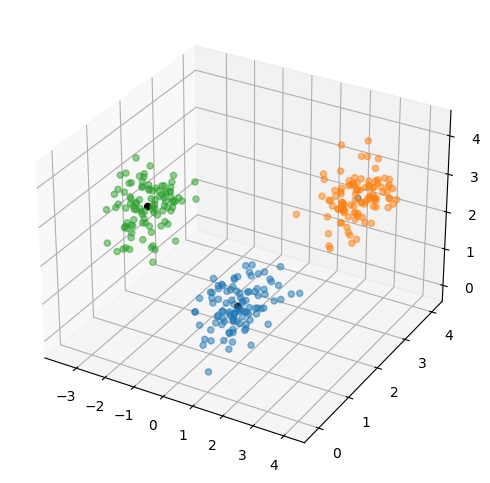
\includegraphics[width=\textwidth]{figures/rs/stitching/clusters_1.png}
        \caption{Three clusters w/ an anchor in each centroid}
         \label{fig:rel_ex_1}
     \end{subfigure}\hfill
      \begin{subfigure}[b]{0.45\textwidth}
         \centering
         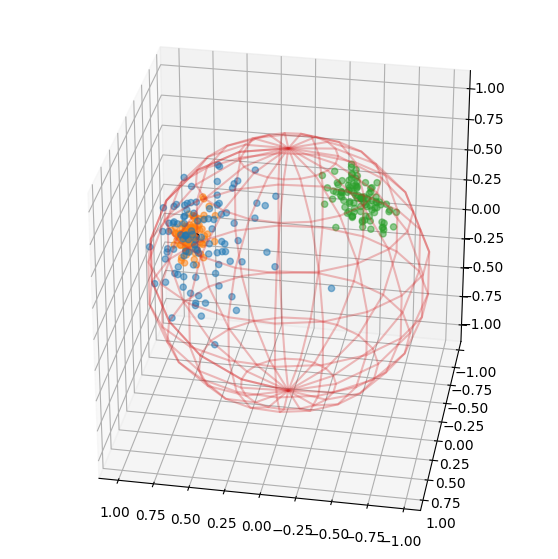
\includegraphics[width=\textwidth]{figures/rs/stitching/clusters_2.png}
        \caption{$L^2$ normalization}
         \label{fig:rel_ex_2}
     \end{subfigure}
     \begin{subfigure}[b]{0.45\textwidth}
         \centering
         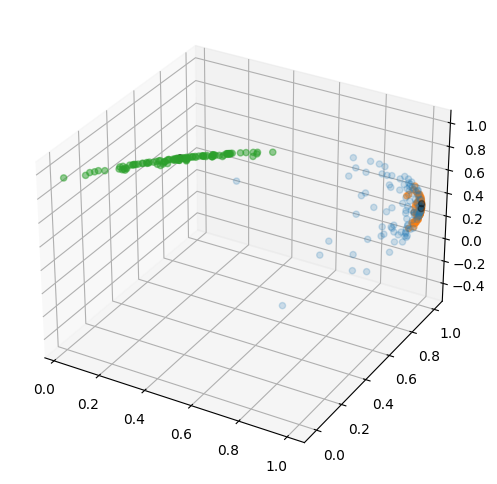
\includegraphics[width=\textwidth]{figures/rs/stitching/clusters_3.png}
        \caption{Cosine similarity}
         \label{fig:rel_ex_3}
     \end{subfigure}
    \caption{Non-cluster preserving relative transformation example}
    \label{fig:rel_ex_bad}
\end{figure}


Therefore, we concluded that applying Hofer's topological regularization to the post-relative space is crucial. However, despite an extensive hyperparameter search, we could still not improve performance. Upon closer examination, we observed that the death times distributions of the post-relative space exhibit a significantly smaller mean than the pre-relative space (see Figure~\ref{fig:distPost}). This implies that when we exclusively apply this loss to the post-relative case, the network discovers an anchor configuration that yields smaller clusters in the post-relative space while preserving the spread of clusters in the pre-relative space. We believe this configuration can lead to information bottlenecks, as compressing the clusters with this nonlinear transformation might cause a loss of expressiveness in the latent space.\\

\begin{figure}[!ht]
    \centering
    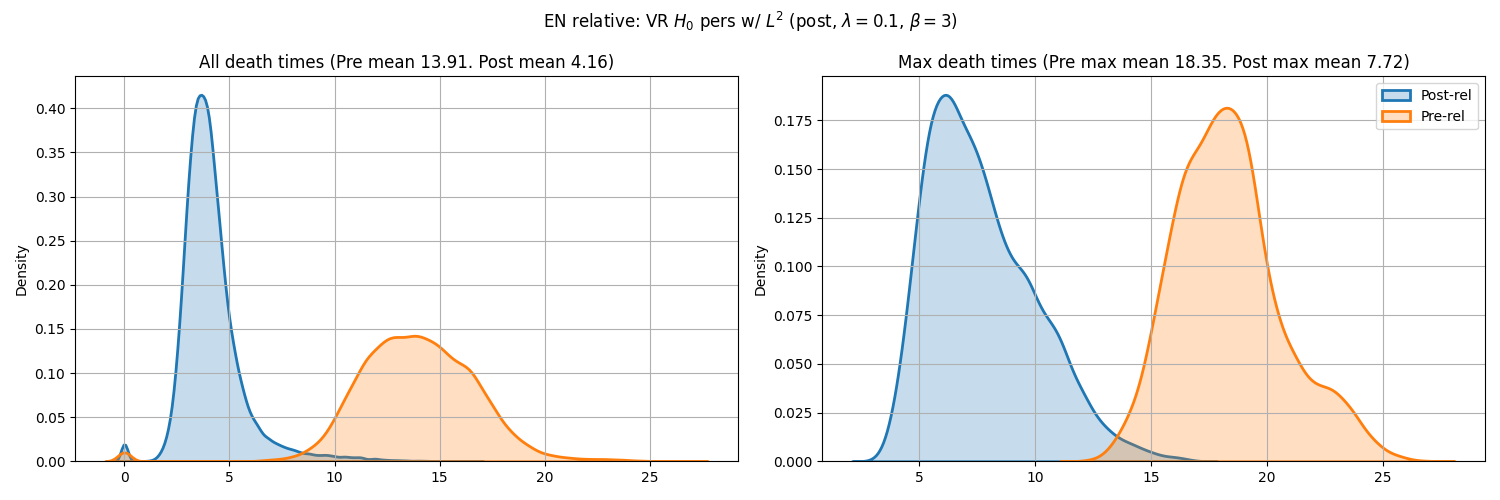
\includegraphics[width=\textwidth]{figures/rs/stitching/en_relative_post_3_seed0.png} 
    \caption{Death times distribution when we apply pre-relative Hofer's topological regularization on the English dataset with $\beta=3$.}
    \label{fig:distPost}
\end{figure}

After further analysis, we discovered that when no regularization is applied, the death times distributions of the network tend to overlap (see Figure~\ref{fig:distVanilla}). This insight led us to favor overlapped death times distributions to preserve $H_0$ homology through the relative transformation. Additionally, this approach addresses the issues we encountered when applying the regularization just before or after the relative transformation.\\

\begin{figure}[ht!]
    \centering
    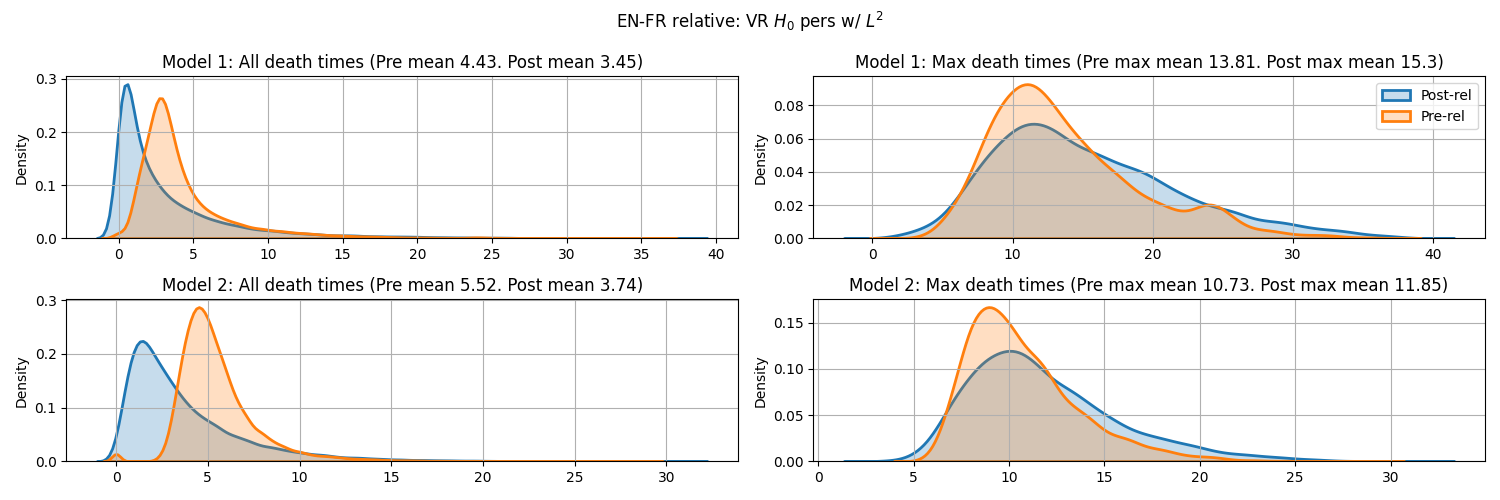
\includegraphics[width=\textwidth]{figures/rs/stitching/en_fr_relative_seed1.png} 
    \caption{Death times distribution without Hofer's topological regularization on the English dataset.}
    \label{fig:distVanilla}
\end{figure}

Following an exhaustive hyperparameter tuning process, we identified that the optimal setup for the absolute case is $\beta=7$ and $\lambda=0.1$ for both the English and French datasets. In the relative case, the best results were obtained by using a linear combination of pre-relative ($0.1$ weight) and post-relative ($0.9$ weight) regularization, with $\beta=3$ and $\lambda=0.02$ for the English case and $\beta=4$ and $\lambda=0.02$ for the French case\footnote{The complete logs of the hyperparameter tuning results and their corresponding death times distributions can be found in the Thesis' GitHub repository.}.\\


\begin{figure}[ht!]
    \centering
    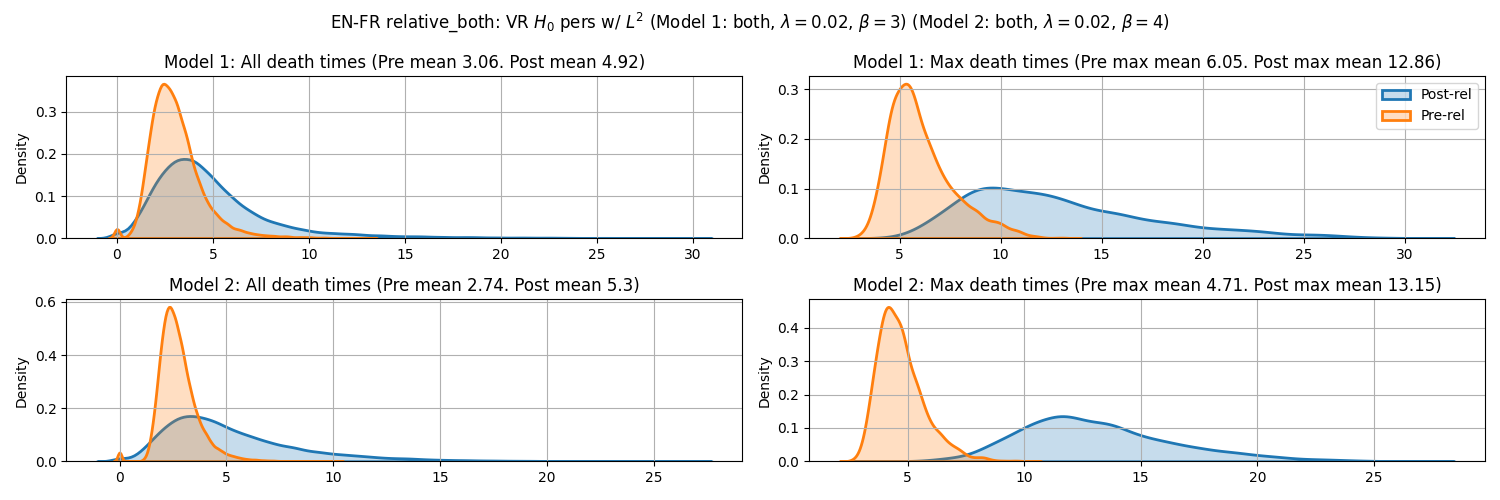
\includegraphics[width=\textwidth]{figures/rs/stitching/en_fr_relative_both_both_both_3_4_seed1.png} 
    \caption{Death times distribution when we apply both pre and post-relative Hofer's topological regularization with $\beta=3$ on the English dataset and $\beta=4$ in the French dataset.}
    \label{fig:distBoth}
\end{figure}


Figure~\ref{fig:distBoth} demonstrates that we successfully encouraged overlapping death times distributions and reduced the maximum death times means. However, it is worth noting that moving the post-relative max distribution proved more challenging. This difficulty arises from the fact that the geometry of the post-relative transformation is influenced by the overall pre-relative latent space and, more significantly, by the images of the anchors. As discussed in Section~\ref{sec:topo_meth}, we compute the anchors' images periodically and do not allow gradients to backpropagate through the anchors\footnote{We do not allow gradients to backprop through the anchors since it would require to virtual increase the sub-batch size by 768.}. Therefore, effecting changes to the post-relative representation is more complex, as it involves adjusting the position of the anchors' images by analyzing the relative transformation of the batch.\\

As shown in Table~\ref{tab:multilingual-linear-topo-unpaired}, employing this topological regularization setup yields better performance in the non-stitching case compared to the new baseline in both the absolute and relative modalities. Furthermore, it outperforms the vanilla dataloader for the non-stitching English model in the relative modality and the French model in the absolute modality. Thus, it is reasonable to assume that with a GPU having much VRAM to accommodate the entire biased batch (without employing gradient accumulation and the debiasing trick), consistently superior results could be achieved compared to the vanilla baseline.\\

\begin{table}[ht!]
\centering
\resizebox{\textwidth}{!}{
\begin{tabular}{clcccccc}
\toprule
   &    & \multicolumn{3}{c}{Absolute} & \multicolumn{3}{c}{Relative} \\
 \cmidrule(lr){3-5} 
 \cmidrule(lr){6-8} 
 Decoder & Encoder & $\text{Acc} \times 100$ & $\text{FScore} \times 100$ & $\text{MAE} \times 100$ & $\text{Acc} \times 100$ & $\text{FScore} \times 100$ & $\text{MAE} \times 100$ \\
\midrule
\multirow{2}{*}{en} & en &  $60.20 \pm 0.88$ &   $59.69 \pm 0.37$ &    $46.33 \pm 0.47$ &  $61.25 \pm 0.24$ &  $61.37 \pm 0.07$ &  $44.50 \pm 0.17$\\
 & fr & $30.04\pm 0.93$ &   $18.56 \pm 1.73$ &  $121.52 \pm 16.07$ &  $50.14 \pm 0.76$ &  $50.55 \pm 0.50$ &  $58.81 \pm 0.16$ \\
&\\
\multirow{2}{*}{fr} & en &  $41.01 \pm 5.53$ &  $29.78 \pm 11.70$ &    $87.95 \pm 7.62$ &  $60.49 \pm 0.78$ &  $60.90 \pm 0.54$ &  $44.96 \pm 0.34$ \\
   & fr &  $51.06 \pm 0.00$ &   $51.81 \pm 0.04$ &    $56.63 \pm 0.01$ &  $51.27 \pm 0.01$ &  $51.71 \pm 0.19$ &  $57.94 \pm 0.74$ \\
\bottomrule
\end{tabular}
}
\caption{Topological regularization (over two random seeds)}
\label{tab:multilingual-linear-topo-unpaired}
\end{table}

The above results demonstrate that with the appropriate setup, we can replicate the results reported in the original Hofer's paper \cite{hofer_densified_2021}, even when using the relative transformation. However, the results of model stitching with topological regularization have not been previously reported. As shown in Table~\ref{tab:multilingual-linear-topo-unpaired}, we achieve improved stitching performance in all stitching combinations and modalities, except for the ``en-fr abs'' case, compared to the new baseline. Moreover, despite observing a performance drop when using the new dataloader with the fix, we surpass the results obtained with the vanilla dataset on stitching for the ``fr-en'' cases in both the relative and absolute modalities.\\

\begin{table}[ht!]
\centering
\resizebox{0.7\textwidth}{!}{
\begin{tabular}{clccc}
\toprule
   &    & \multicolumn{3}{c}{Relative} \\
 \cmidrule(lr){3-5} 
 Decoder & Encoder & $\text{Acc} \times 100$ & $\text{FScore} \times 100$ & $\text{MAE} \times 100$ \\
\midrule
\multirow{2}{*}{en} & en &  $61.25 \pm 0.24$ &  $61.37 \pm 0.07$ &  $44.50 \pm 0.17$ \\
   & fr &  $\bm{50.90 \pm 0.65}$ &  $\bm{51.50 \pm 0.66}$ &  $\bm{57.27 \pm 0.07}$ \\
&\\
\multirow{2}{*}{fr} & en &  $\bm{60.87 \pm 0.95}$ &  $\bm{61.27 \pm 0.77}$ &  $\bm{44.56 \pm 0.71}$ \\
   & fr &  $50.11 \pm 0.38$ &  $50.58 \pm 0.79$ &  $57.78 \pm 0.14$ \\
\bottomrule
\end{tabular}
}
\caption{Topological reg. w/ matched params (over two random seeds)}
\label{tab:multilingual-linear-topo-paired}
\end{table}

Additionally, Table~\ref{tab:multilingual-linear-topo-paired} reveals that we can enhance stitching performance by selecting the same $\beta$ parameter for topological regularization (i.e., using $\beta=4$ for the French case). However, this impacts non-stitching performance, as the optimal hyperparameter choice of $\beta=3$ is no longer used. This observation is logical since a specific hyperparameter choice will yield the best results for a given dataset during network training. Nevertheless, for stitching purposes, it is preferable to impose consistent condensation, increasing the possibility that class clusters reside within the decision boundary of the other classifier.

\begin{mathNote}
Hofer's topological regularization generally does not outperform early stopping in terms of non-stitching performance. However, in the ``fr-en'' stitching case, we achieve better results than early stopping (see Tables~\ref{tab:multilingual-linear-vanilla-stop},~\ref{tab:multilingual-linear-biased-stop}).
\end{mathNote}

The reason why we could not successfully apply Hofer's topological regularization to the Spanish case as well as why the ``en-fr'' stitching case does not perform as well as ``fr-en'', will be discussed in Section~\ref{sec:more_topo}.\\

As outlined in Section~\ref{sec:topo_meth}, utilizing $L^\infty$ in the post-relative space offers certain advantages. In this section, we will demonstrate how it can be beneficial for hyperparameter selection. In previous experiments, the approach involved computing the death times distribution and conducting a grid search based on values such as $0.3\times \text{post\_mean}$, $0.5\times \text{post\_mean}$, $0.6\times \text{post\_mean}$, $0.3\times \text{post\_max\_mean}$, $0.5\times \text{post\_max\_mean}$, and $0.6\times \text{post\_max\_mean}$. However, a new approach can be adopted:
\begin{enumerate}
    \item Compute the death times distributions using the $L^2$ in the pre-relative space and $L^\infty$ in the post-relative space. As an example, in Figure~\ref{fig:distMix}, we can see the resulting distributions for the English relative case.

    \item Determine the approximate spread of the cluster using
    \[\theta_{og} = 180 \arccos(1-\text{post\_mean}).\]
    In the previous example, $\theta_{og}$ is approximately $36^{\circ}$.
    
    \item Conduct a grid search for $\theta \in [\tau_1 \theta_{og}, \tau_2\theta_{og}]$, where $\tau_1\geq 0$ and $\tau_2> 0$, with a specified step size $\delta \theta$. Set $\beta_{post} = 1-\cos(\pi \theta / 180)$.
\end{enumerate}

\begin{figure}[!ht]
    \centering
    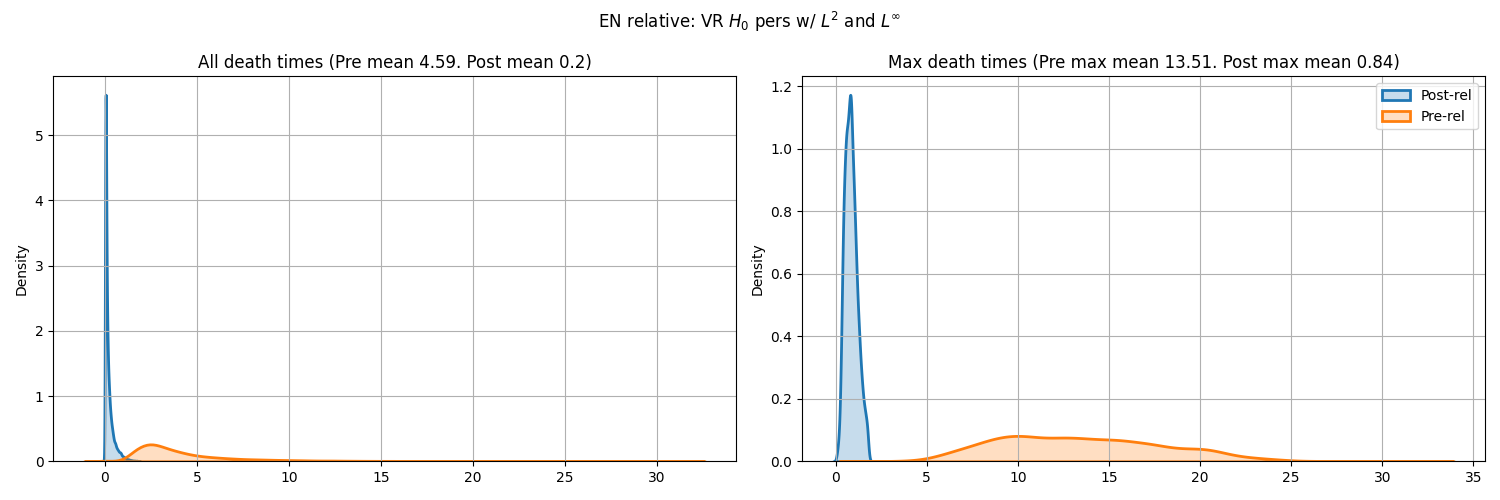
\includegraphics[width=\textwidth]{figures/rs/stitching/mix_en_relative_seed0.png} 
    \caption{Death times distribution on the English dataset. $L^2$ is used in the pre-relative space and $L^\infty$ in the post-relative space.}
    \label{fig:distMix}
\end{figure}

Therefore, we performed a grid search on $\theta \in [5^{\circ}, 30^{\circ}]$ with a step size of $\delta \theta = 5^{\circ}$, while keeping $\beta_{pre}$ fixed at 3. Surprisingly, for $\theta = 25^{\circ}$, we achieved better performance compared to using $L^2$ with $\beta_{post} = 3$ ($61.48$ FScore $\times 100$). Hence, this result serves as a proof of concept for the potential exploration of different metrics when employing Hofer's topological regularization\footnote{Due to time limitations, we were not able to fully explore the $L^\infty$ case to be able to produce a table with proper hyperparameter tuning as we did for the $L^2$ cases.}.







\end{document}